\documentclass[a4paper,14pt]{article}
\usepackage{float}
\usepackage{extsizes}
\usepackage{amsmath}
\usepackage{amssymb}
\everymath{\displaystyle}
\usepackage{geometry}
\usepackage{fancyhdr}
\usepackage{multicol}
\usepackage{graphicx}
\usepackage[brazil]{babel}
\usepackage[shortlabels]{enumitem}
\usepackage{cancel}
\columnsep=2cm
\hoffset=0cm
\textwidth=8cm
\setlength{\columnseprule}{.1pt}
\setlength{\columnsep}{2cm}
\renewcommand{\headrulewidth}{0pt}
\geometry{top=1in, bottom=1in, left=0.7in, right=0.5in}

\pagestyle{fancy}
\fancyhf{}
\fancyfoot[C]{\thepage}

\begin{document}
	
	\noindent\textbf{6FMA55~Matemática} 
	
	\begin{center}Números Decimais (Versão estudante)
	\end{center}
	
	\noindent\textbf{Nome:} \underline{\hspace{10cm}}
	\noindent\textbf{Data:} \underline{\hspace{4cm}}
	
	%\section*{Questões de Matemática}
	
	
    \begin{multicols}{2}
    	\begin{enumerate}
    		\item Escreva como se lê:
	    	\begin{enumerate}[a)]
				\item $\frac{1}{100}$ \\\\
				\item $0,001$ \\\\
				\item $\frac{1}{10000}$ \\\\
	        \end{enumerate}
        	\item Calcule, escreva o resultado na forma decimal e diga como se lê:
        	\begin{enumerate}[a)]
        		\item $4 \cdot 0,1 = $ \\\\
        		\item $0,1 \cdot 6 = $ \\\\
        		\item $7 \cdot \frac{1}{10} = $ \\\\
        	\end{enumerate}
            \item Escreva o resultado:
            \begin{enumerate}[a)]
            	\item $0,1 + 0,1 + 0,1 + 0,1 + 0,1 + 0,1$ \\\\
            	\item $8 \cdot 0,1$ \\\\
            	\item $14 \cdot 0,1$ \\\\
            	\item $0,01 \cdot 82$ \\\\
            \end{enumerate}
        	\item Escreva o número\\\\
        	$2 + \frac{5}{10} + \frac{9}{100} + \frac{6}{1000} + \frac{3}{10000}$ \\\\
        	na forma decimal.\\\\
        	\item Escreva o número 6,509 como soma de frações e inteiros.\\\\
        	\item Complete com os nomes das posições dos algarismos.
        	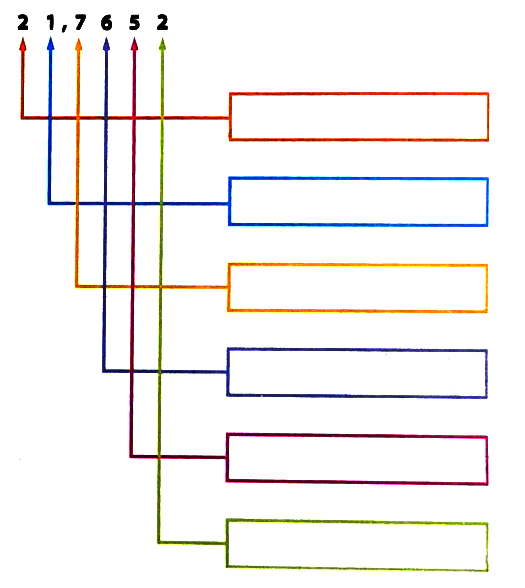
\includegraphics[width=1\linewidth]{6FMA55_imagens/imagem0}
        	
        	\item Assinale V (verdadeiro) ou F (falso).\\
        	Carlinhos tem 1,58 metro de altura. Ele poderia dizer que mede:
        	\begin{enumerate}[a)]
        		\item (~~) 158 centímetros (ou 158 centésimos de metro).
        		\item (~~) 1 metro, 5 decímetros e 8 centímetros.
        		\item (~~) 1 vírgula 58 metro.
        	\end{enumerate}
        	\item Determine o decimal que representa a parte destacada em cada um dos itens abaixo:
        	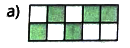
\includegraphics[width=1\linewidth]{6FMA55_imagens/imagem1}
        	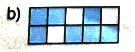
\includegraphics[width=1\linewidth]{6FMA55_imagens/imagem2}
        	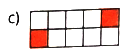
\includegraphics[width=1\linewidth]{6FMA55_imagens/imagem3}
        	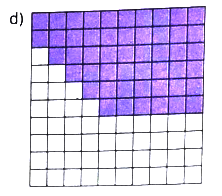
\includegraphics[width=1\linewidth]{6FMA55_imagens/imagem4}
        	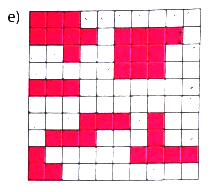
\includegraphics[width=1\linewidth]{6FMA55_imagens/imagem5}
        	\item Localize na reta os números 0,6; 1,7 e 2,3.\\ 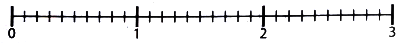
\includegraphics[width=1.1\linewidth]{6FMA55_imagens/imagem6}
        	\item Qual dos decimais na roda abaixo:\\
        	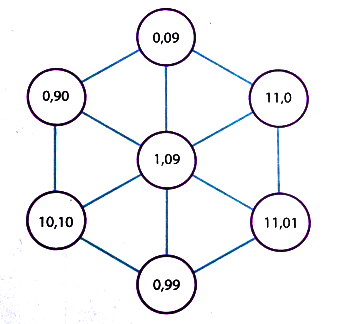
\includegraphics[width=1\linewidth]{6FMA55_imagens/imagem7}
        	\begin{enumerate}[a)]
        		\item é o maior?
        		\item é o menor?
        	\end{enumerate}
        	\item Carla tem 1,682 m de altura. Se 1 m vale 100 cm, qual é sua altura em cm?
        \end{enumerate}
    $~$ \\ $~$ \\ $~$ \\ $~$ \\ $~$ \\
    \end{multicols}
\end{document}